\documentclass[12pt]{article}

\begin{document}
\section{Conversor DC-DC Buck}
\subsection{Análise teórica}
Este capitulo tem como objetivo analisar o conversor DC-DC Buck. Assim, será determinada a função transferência $\frac{V_{out}}{V_i}$ do conversor, que permitirá chegar a um fator de conversão, bem como a eficiência do mesmo. Esta analise será feita sem ter em conta as capacidades parasitas.
O conversor Buck está representado na figura  \ref{fig:Nucleo_do_conversor_DC-DC_Buck}.
\begin{figure}[htbp]
	\centering
	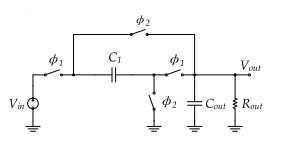
\includegraphics[height=2.5cm]{Buck}
	\caption{Núcleo do conversor DC-DC Buck}
	\label{fig:Nucleo_do_conversor_DC-DC_Buck}
\end{figure}

A análise do conversor será realizada em três instantes, em que cada um está associado a uma fase. Se o circuito estiver a funcionar na fase 1 ($\phi_1$) obtém-se o circuito representado na figura \ref{fig:Fase1}, mas se estiver a funcionar na fase 2 ($\phi_2$) obtém-se o circuito da figura \ref{fig:Fase2}.
	
\begin{figure}[htbp]
\centering
\begin{minipage}{.5\textwidth}
	\centering
	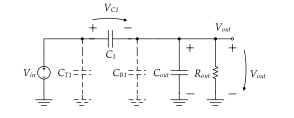
\includegraphics[width=1.0\linewidth, height=2.5cm]{Fase1}
	\caption{Fase 1 ($\phi_1$)}
	\label{fig:Fase1}
\end{minipage}%
\begin{minipage}{.5\textwidth}
	\centering
	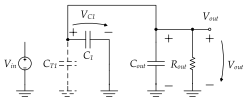
\includegraphics[width=1.0\linewidth, height=2.5cm]{Fase2}
	\caption{Fase 2 ($\phi_2$)}
	\label{fig:Fase2}
\end{minipage}
\end{figure}

De forma a obter a relação $\frac{V_{out}}{V_i}$ considera-se que existe conservação de carga entre fases. Em ambos os casos existe conservação de carga no nó de saída e considerando o seguinte andamento temporal (figura \ref{fig:Andamento temporal}).

\begin{figure}[h]
	\centering
	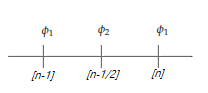
\includegraphics[height=2.5cm]{andamentotemporal}
	\caption{Andamento temporal}
	\label{fig:Andamento temporal}
\end{figure}
Considerando a conservação de carga da fase 1 para a fase 2 ($\phi_1 \rightarrow \phi_2$) obtém-se a seguinte equação.
\vspace{5mm}

{\footnotesize\begin{equation}
\label{eq:Fase1to2}
Q^{\phi_2}_{C_1} + Q^{\phi_2}_{C_{out}} + \Delta Q_{Rout} = Q^{\phi_1}_{C_1} + Q^{\phi_1}_{C_{out}} 
\end{equation}}
\vspace{5mm}

Tendo em consideração que $\Delta Q_{Rout} = \frac{T_{clk} }{2}I_{out}$ a equação \ref{eq:Fase1to2} pode ser escrita da seguinte forma:

{\footnotesize\begin{equation}
\label{eq:Fase1to2s}
V_{out}[n-\frac{1}{2}]C_1 + V_{out}[n-\frac{1}{2}]C_{out} +  V_{out}[n-\frac{1}{2}](\frac{T_{clk} }{2}\frac{1}{R_{out}})=(V_i-V_{out}[n-1])C_1 + V_{out}[n-1]C_{out}
\end{equation}}
\vspace{5mm}

Considerando agora a conservação de carga da fase 2 para a fase 1 ($\phi_2 \rightarrow \phi_1$) obtém-se a seguinte equação.


{\footnotesize \begin{equation}
  \begin{array}{ccc}
  -Q^{\phi_1}_{C_1} + Q^{\phi_1}_{C_{out}} + \Delta Q_{Rout} = -Q^{\phi_2}_{C_1} + Q^{\phi_2}_{C_{out}} \\[1em]
  -(V_i-V_{out}[n])C_1+V_{out}[n]C{out}+V_{out}[n](\frac{T_{clk} }{2}\frac{1}{R_{out}}) = - V_{out}[n-\frac{1}{2}]C_1+V_{out}[n-\frac{1}{2}]C_{out} 
   \end{array}
   \label{eq:Fase2to1}
\end{equation}}
\vspace{5mm} 

Resolvendo a equação \ref{eq:Fase2to1} em ordem a $V_{out}[n-\frac{1}{2}]$ e substituindo na equação \ref{eq:Fase1to2s} obtém-se a seguinte expressão de $\frac{V_{out}}{V_i}$.
{\footnotesize\begin{equation}
\label{eq:Buck(vo/vi)}
\frac{V_{out}}{V_i} = \frac{C_1(2 + \frac{T_{clk}}{2}\frac{1}{C{out}R_{out}})}{4C_1+ \frac{C_1T{clk}}{C{out}R_{out}} +  \frac{T_{clk}}{R_{out}} + \frac{T{clk}^2}{4R_{out}^2C_{out}} }
\end{equation}}
\vspace{5mm} 

Considerando $C_{out}>> C_1$ e que $F_{clk} = \frac{1}{T{clk}}$ obtém-se:
\vspace{5mm}     

{\footnotesize\begin{equation}
\label{eq:Buck(vo/vi)ap}
\frac{V_{out}}{V_i} = \frac{2F_{clk}R_{out}C_1}{4F_{clk}R_{out}C_1+ 1}
\end{equation}}
\vspace{5mm}  

Como $4F_{clk}R_{out}C_1 > 1$ então: 

{\footnotesize\begin{equation}
\label{eq:Buck(vo/vi)f}
\frac{V_{out}}{V_i} = \frac{1}{2}
\end{equation}}
\vspace{5mm}
  
Assim sendo, a razão de conversão do conversor é de $\frac{1}{2}$.

Através da equação \ref{eq:Buck(vo/vi)ap} é possível chegar á $F_{clk}$ do conversor.
{\footnotesize\begin{equation}
\label{eq:FBuck(vo/vi)}
F_{clk}=\frac{V_{out}}{2R_{out}C_{1}(V_i-2V_{out})}
\end{equation}}
\vspace{5mm}

A eficiência do conversor é dada por: $\eta = \frac{P_{out}}{P_{i}}$ onde $P_{out} = V_{out}I_{out}$ e $P_{in} = V_{i}I_{i}$
{\footnotesize\begin{equation}
\label{eq:EfBuck(vo/vi)}
\eta = \frac{P_{out}}{P_{in}} = \frac{ V_{out}I_{out}}{ V_iI_i} = \frac{|V_{out}(\Delta Q^{\phi_1}_{out} + \Delta Q^{\phi_2}_{out})F_{clk}|}{{|V_i(\Delta Q^{\phi_1}_{i} + \Delta Q^{\phi_2}_{i})F_{clk}|}}
\end{equation}}

De forma a calcular a variação da carga à saída e à entrada nas duas fases, recorreu-se às figuras \ref{fig:Ef1} e \ref{fig:Ef2}. 

\begin{figure}[htbp]
\centering
\begin{minipage}{.5\textwidth}
	\centering
	\includegraphics[width=0.8\linewidth, height=2.5cm]{Ef1}
	\caption{Fase 1 ($\phi_1$)}
	\label{fig:Ef1}
\end{minipage}%
\begin{minipage}{.5\textwidth}
	\centering
	\includegraphics[width=0.8\linewidth, height=2.5cm]{Ef2}
	\caption{Fase 2 ($\phi_2$)}
	\label{fig:Ef2}
\end{minipage}
\end{figure}

Considerando a conservação de carga da fase 1 para a fase 2 ($\phi_1 \rightarrow \phi_2$) é possível retirar a variação da carga á entrada e á saída da fase 2.
\vspace{5mm}

Nó de saída:

{\footnotesize \begin{equation}  
\label{eq:Variao2}
\begin{array}{ccc}
    Q^{\phi_2}_{C_1} + \Delta Q^{\phi_2}_{out} &=& Q^{\phi_1}_{C_1}\\  [1em]        
    V_{out}C_1+\Delta Q^{\phi_2}_{out} &=& (V_i-V_{out})C_1 \\[1em]
    \Delta Q^{\phi_2}_{out} &=& (V_i - 2V_{out})C_1  
  \end{array}
  \end{equation}}
  \vspace{5mm}
  
   No nó de entrada a $\Delta Q^{\phi_2}_{i} = 0$.
   \vspace{5mm}
   
   Considerando agora a conservação de carga da fase 2 para a fase 1 ($\phi_2 \rightarrow \phi_1$) é possível retirar a variação da carga á entrada e á saída da fase 1.
   \vspace{5mm}

Nó de saída:

{\footnotesize \begin{equation}  
\label{eq:Variao1s}
\begin{array}{ccc}
   - Q^{\phi_1}_{C_1} + \Delta Q^{\phi_1}_{out} &=& -Q^{\phi_2}_{C_1}\\  [1em]        
   -(V_i-V_{out})C_1+\Delta Q^{\phi_1}_{out} &=& -V_{out}C_1 \\[1em]
    \Delta Q^{\phi_1}_{out} &=& (V_i - 2V_{out})C_1
  \end{array}
  \end{equation}}
  \vspace{5mm}

Nó de entrada:

{\footnotesize \begin{equation} 
\label{eq:Variao1i}
\begin{array}{ccc}
   Q^{\phi_1}_{C_1} + \Delta Q^{\phi_1}_{i} &=& Q^{\phi_1}_{C_1}\\  [1em]        
   (V_i-V_{out})C_1+\Delta Q^{\phi_1}_{i} &=& V_{out}C_1 \\[1em]
    \Delta Q^{\phi_1}_{i} &=& ( 2V_{out}-V_i)C_1
  \end{array}
  \end{equation}}
  \vspace{5mm}

Substituindo a equação \ref{eq:EfBuck(vo/vi)} pelas expressões obtidas para a variação na carga á entrada e á saída das duas fases obtém-se:

{\footnotesize \begin{equation}
\label{eq:EfBuck(vo/vi)_final}
\begin{array}{cc}
\eta = \frac{|V_{out}((V_i - 2V_{out})C_1 + (V_i - 2V_{out})C_1  )F_{clk}|}{{|V_i(( 2V_{out}-V_i)C_1 + 0)F_{clk}|}} = |-\frac{2V_{out}}{V_i}|\\ [1em]
\eta =\frac{2V_{out}}{V_i}
\end{array}
\end{equation}}
\subsection{Dimensionamento dos componentes}

Para dimensionar corretamente o conversor, começou-se por escolher o tipo de transístores a utilizar, optando assim que $S_1$ seria PMOS visto que para o conversor começar a trabalhar necessita de uma tensão mais elevada e que $S_4$ seria NMOS para puxar essa tensão. Quanto aos outros dois transístores estes podiam ser tanto NMOS como PMOS, assim optou-se por utilizar uma configuração Transmission Gate.

Quando o interruptor está fechado existe uma resistência intrínseca  denominada por $R_{on}$ na figura \ref{fig:Fase1Ron} e na figura  \ref{fig:Fase2Ron} está representada a resistência $R_{on}$ para a fase ($\phi_1$) e ($\phi_2$).7  
\begin{figure}[htbp]
\centering
\begin{minipage}{.5\textwidth}
	\centering
	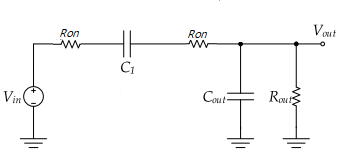
\includegraphics[width=0.8\linewidth, height=2.5cm]{Fase1Ron}
	\caption{Fase 1 ($\phi_1$) com $R_{on}$}
	\label{fig:Fase1Ron}
\end{minipage}%
\begin{minipage}{.5\textwidth}
	\centering
	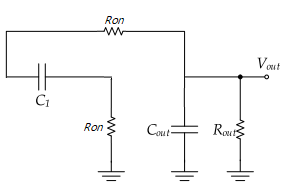
\includegraphics[width=0.8\linewidth, height=2.5cm]{Fase2Ron}
	\caption{Fase 2 ($\phi_2$) com $R_{on}$}
	\label{fig:Fase2Ron}
\end{minipage}
\end{figure}

Considerando quando o circuito da figura \ref{fig:Fase1Ron} está a funcionar, na fase 1 verifica-se que estamos perante um circuito RC de segunda ordem. Contudo este pode ser aproximado a um de primeira ordem considerando os valores de $R_{out}$ e $C_{out}$ elevados face ao valor de $R_{on}$ (resistência do interruptor) e $C_{1}$, respetivamente. Assim, a constante de tempo ($\tau$) associada à carga e descarga do condensador é dada por $2R_{on}C_1$, assumindo um erro de $1\%$ no fator de conversão é possível chegar ao valor de $R_{on}$ e posteriormente ao valor de W do transístor uma vez que $L = 120 [nm]$.
Realizando uma análise semelhante quando o circuito funciona na fase 2 verifica-se que a constante de tempo não sofre alteração. 

Com base nas especificações:

\begin{itemize}
\item \begin{center} $V_i = 1.2$ [V] \end{center}
\item \begin{center} $C_1 = 0.5 $[nF] \end{center}
\item \begin{center} $R_{out} = 500 $[$\Omega$] \end{center}
\end{itemize}

E tendo em conta que $V_{out}$ é metade do valor de entrada considerou-se $V_{out}$ = 0.58 [V]. Assim pela equação \ref{eq:FBuck(vo/vi)} chegou-se a um valor de $F_{CLK} = 30$ [MHz].
Sabendo que a tensão no condensador para um circuito de primeira ordem é dado pela equação \ref{eq:tensaonocondensador} e o andamento temporal de carga no condensador está representado na figura \ref{fig:tensaonoc}, é possível calcular um erro de 1 \% face ao valor máximo de carga. Considerando que $V_f  = 0 $ a equação \ref{eq:tensaonocondensador} simplifica-se para $\frac{V_{out}}{V_i} =  e^{-(\frac{T}{\tau})} = erro$ sendo a carga máxima dada quando $T = \frac{T_{CLK}}{2}$.


\begin{figure}[htbp]
	\centering
	\begin{minipage}{.5\textwidth}
		\centering
		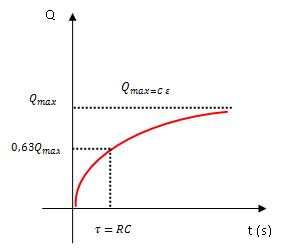
\includegraphics[width=0.6\linewidth, height=2.5cm]{tensaonocondensador}
		\caption{Andamento temporal de carga do condensador}
		\label{fig:tensaonoc}
	\end{minipage}%
	\begin{minipage}{.5\textwidth}
		\centering
		{\footnotesize \begin{equation}
			\label{eq:tensaonocondensador}
			 V_c = V_f-(V_f-V_i)e^{-(\frac{T}{\tau})}
		\end{equation}} 
	\end{minipage}
\end{figure}

Com base na explicação feita anteriormente, estamos em condições de retirar o valor de $R_{on}$.

{\footnotesize \begin{equation}
\label{eq:Ron}
\begin{array}{cc}
erro  = e^{-(\frac{T}{\tau})} \\ [1em]
erro = e^{-(\frac{T_{CLK}}{2(2R_{on}C_1)})} \\ [1em]
R_{on} = -\frac{T_{CLK}}{4C1ln(erro)}
\end{array}
\end{equation}}

Através da equação \ref{eq:Ron} chegou-se a um valor de $R_{on}$ de 3.74 $[\Omega]$. 
A resistência também pode ser calculada a partir da equação \ref{eq:RonT}. Contudo, já tendo este valor é possível chegar ao valor de W para cada tipo de interruptor através de uma parametrização no programa Cadance, onde se considera $\frac{L}{K(V_{(GS/SG)} - V_{(THN/THP)}} = K_r$ 

{\footnotesize \begin{equation}
	\label{eq:RonT}
	R_{on}= \frac{L}{WK(V_{(GS/SG)} - V_{(THN/THP)})}
\end{equation}}

O esquemático para realizar a parametrização encontra-se representado na figura \ref{fig:esquematicop}. O exemplo apresentado é para o interruptor $S_4$ que irá ser implementado com um transistor NMOS e por este motivo coloca-se uma tensão de 1.2 [V] na gate. Através do programa Cadance obtém-se um gráfico representado na figura \ref{fig:graficoRon} que relaciona $R_{on}$ com W, a variação do eixo das ordenadas corresponde a $K_r$ mencionado em cima. Para os restantes interruptores o raciocínio é semelhante, tendo em atenção os valores a colocar nas fonte de tensão $V_0$ e  $V_1$. Na tabela \ref{tab:dimensionamento} encontra-se o dimensionamento para todos os interruptores considerando um erro de $1\%$.



\begin{figure}[htbp]
	\centering
	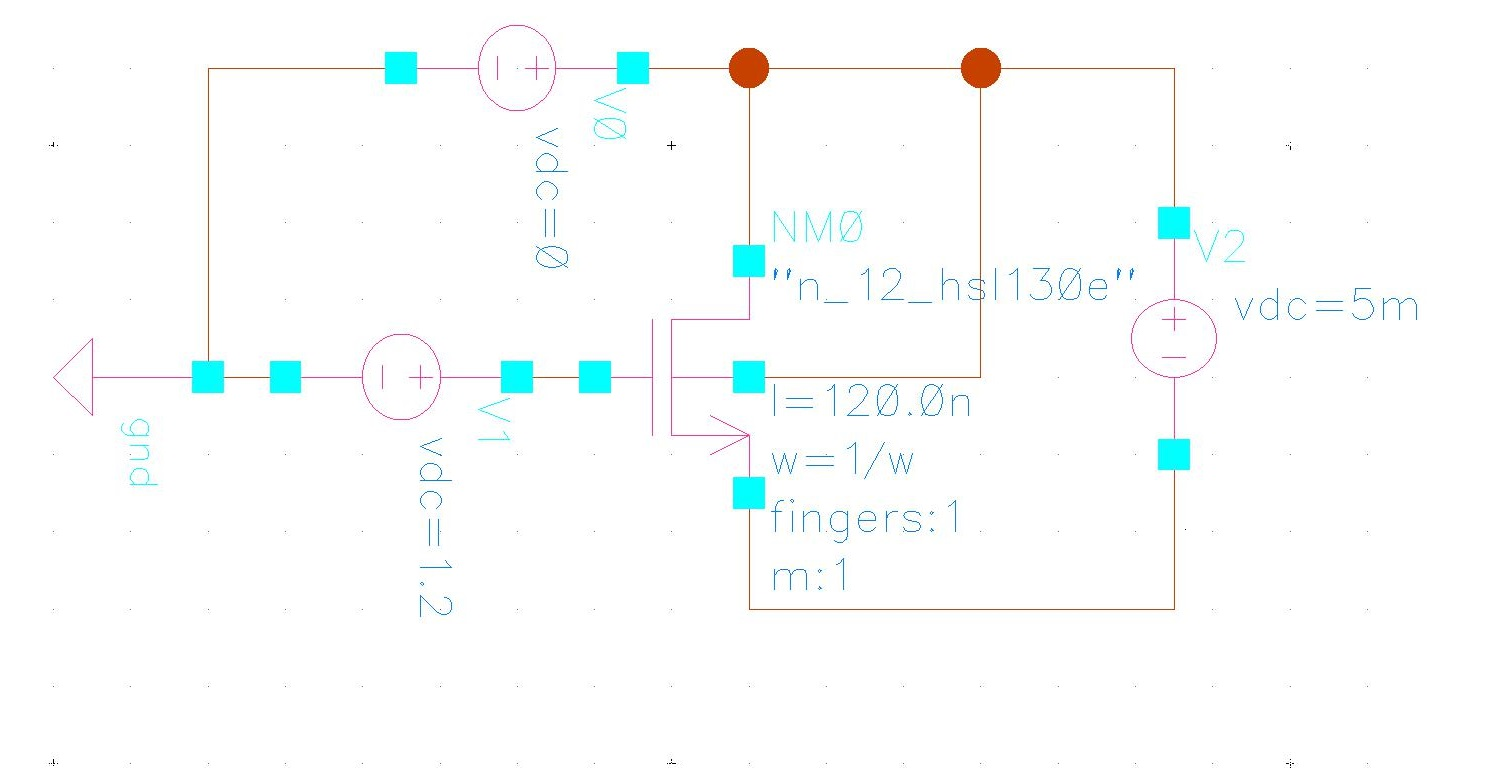
\includegraphics[width=0.5\linewidth, height=4cm]{ParamNmos}
	\caption{Parametrização do transístor NMOS}
	\label{fig:esquematicop}
\end{figure}
\begin{figure}[htbp]
	\centering
	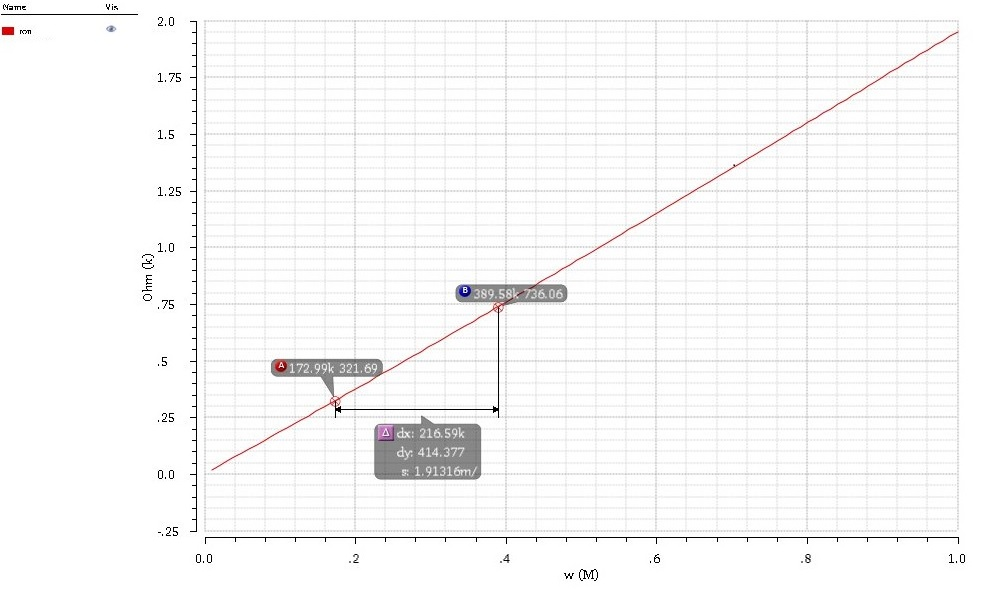
\includegraphics[width=0.7\linewidth, height=6cm]{ParamNo}
	\caption{$R_{on}$ em função de W}
	\label{fig:graficoRon}
\end{figure}


\begin{table}[hbtp]
\centering
\caption{Dimensionamento de interruptores}
\label{tab:dimensionamento}
\begin{tabular}{|c|c|c|c|c|c|c|c|}
\hline
Interruptores & Tipo                      & $V_0$ $[V]$  &$V_1$ $[V]$  & $Ron$ [$\Omega$]    & $Kr$        & W [$\mu m$]     & $L$ $[nm]$   \\ \hline
S1            & PMOS                     & 1.2 & 0   & 3.7439 & 0.0020     & 527.95 & 120 \\ \hline
S2/S3         & T. Gate - PMOS & 1.2 & 0.6 & 7.4878 & 0.0053     & 117.52 & 120 \\ \hline
S2/S3         & T. Gate - NMOS & 0.6 & 1.2 & 7.4878 & 0.0012     & 156.06 & 120 \\ \hline
S4            & NMOS                     & 0   & 1.2 & 3.7439 & 0.0004 & 708.58 & 120 \\ \hline
\end{tabular}
\end{table}
\vspace{5mm}
\subsection{Simulação do núcleo do conversor}
Nesta secção serão apresentados os resultados obtido para o núcleo do conversor. Na figura \ref{fig:DC_GF_esquematico} encontra-se o circuito utilizado na simulação, as fases 1 ($\phi_1$) e 2 ($\phi_2$) foram implementadas através de uma fonte $V_{pulse}$ em que a fase ($\phi_1$) é o inverso da fase 2 ($\phi_2$).
\vspace{5mm}

\begin{figure}[h]
	\centering
	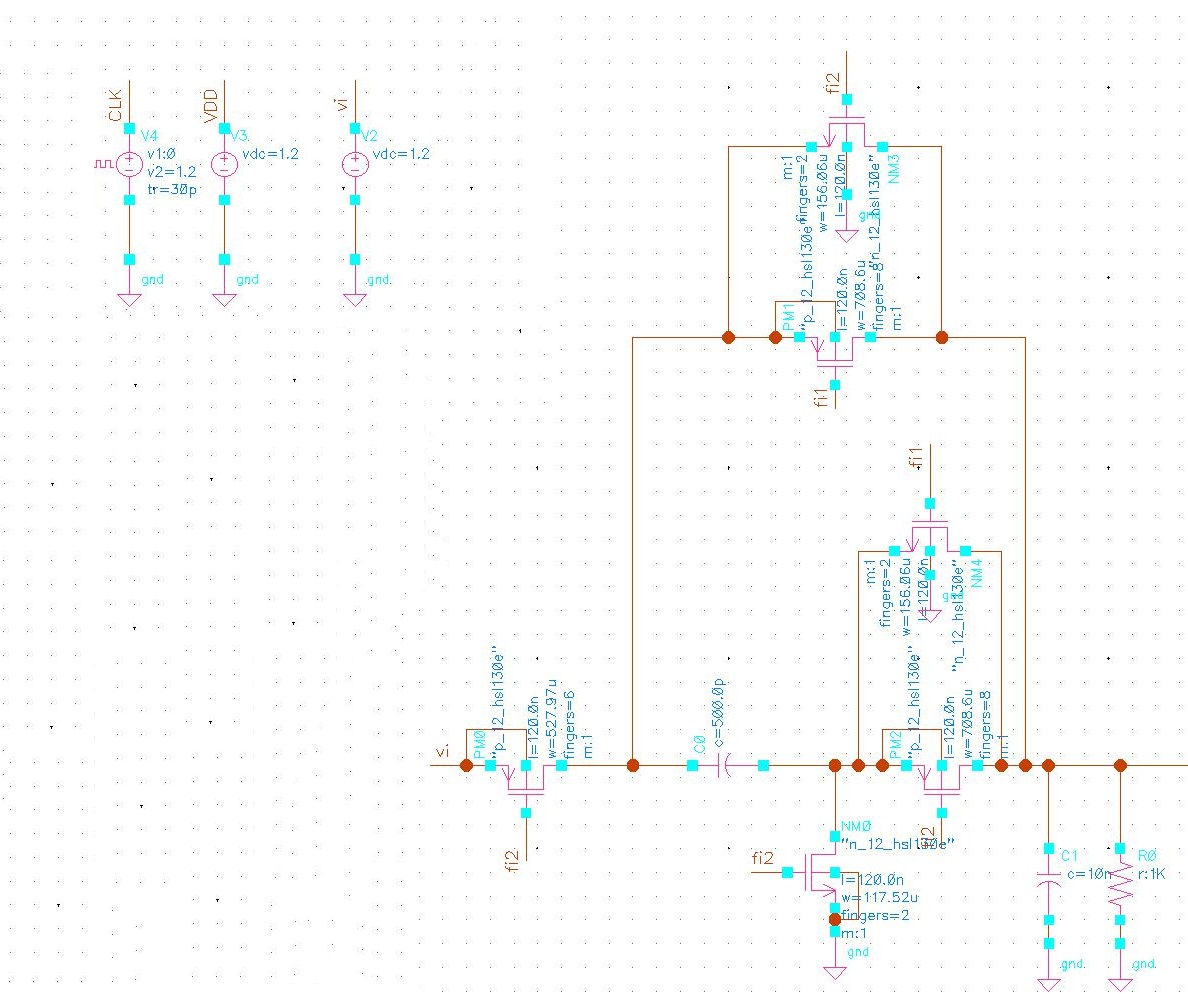
\includegraphics[height=10cm]{DC_GF_esquematico}
	\caption{Circuito do núcleo do conversor}
	\label{fig:DC_GF_esquematico}
\end{figure}
\vspace{5mm}


Numa primeira análise considerou-se que $C_{out}$ = 10 [pF] e $R_{out} = 500$ $[\Omega]$, contudo a onda à saída encontrava-se cerca de 300 [mV] abaixo do valor pretendido. Ao realizar vários testes observou-se que ao aumentar $R_{out}$ o tempo de descarga do condensador diminuía e por sua vez quanto maior fosse o valor de $C_{out}$ menor era o valor de ripple e o valor de tensão à saída também diminuía significativamente. De forma a ter um valor de ripple o mais baixo possível e o valor de saída perto 600 [mV], optou-se por aumentar  $C_{out}$ = 10 [nF] e $R_{out} = 1$ $[k\Omega]$. 

Os resultados obtidos encontram-se representados na figura \ref{fig:onda_saida_com_ripple}.

A tensão à saída do conversor é de 580.21[mV] tendo um valor de ripple de 0.841 [mV], sendo estes valores bastante aceitáveis para o núcleo do conversor.
\break
\break

\begin{figure}[hbtp]
	\centering
	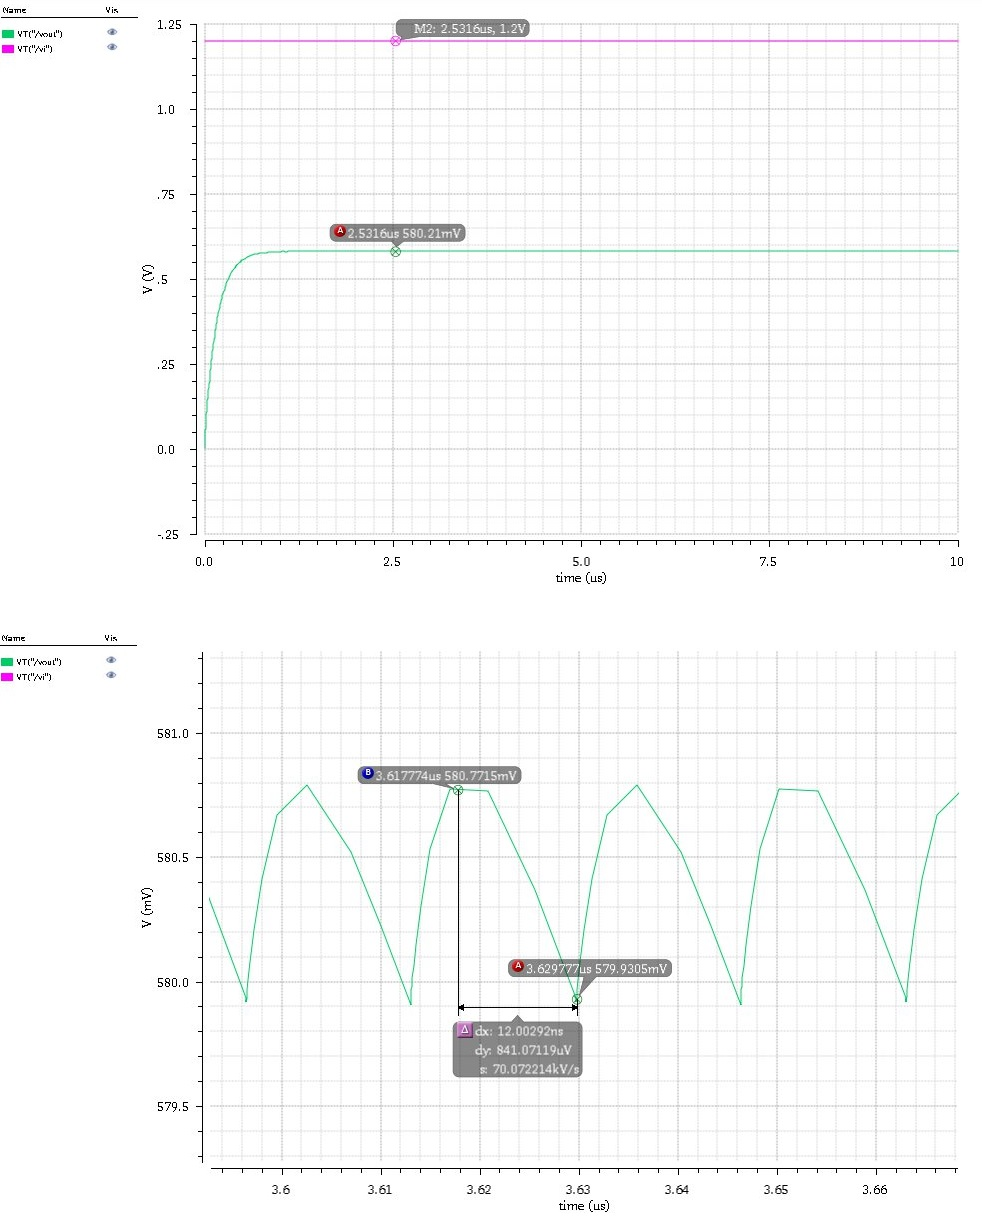
\includegraphics[height=18cm]{DCDC_von_vout_ripple}
	\caption{Onda à entrada (verde) e à saída (Rosa) do conversor}
	\label{fig:onda_saida_com_ripple} 
\end{figure}  



   
%\begin{cases}
%Q^{\phi_2}_{C_1} + \Delta Q^{\phi_2}_{out}=Q^{\phi_1}_{C_1}
%\\
%0.3 & \text{if } u=1,
%\\
%0.6 & \text{if } u=2.
%\end{cases}

%\begin{equation}
%  \begin{array}{lll}
%    a + b + c = d \\        
%    e + f =  g \\        
%    h =i
%  \end{array}
%\end{equation}

\end{document} 